%==============================================================================
\section{Simulation Input}
\label{sec:sim_input}
%==============================================================================

% \begin{figure}
%  \centering
%  \includegraphics[width=0.495\linewidth]{figures/a_eff_plot.pdf}
%  \includegraphics[width=0.495\linewidth]{figures/coszen_dependence.pdf}
%  \caption{Effective areas for all relevant neutrino interactions. Shown are
%   energy (left)  and zenith (right) dependence.}
% \label{fig:aeffs}
% \end{figure}

The effective areas are
extracted from PINGU Monte Carlo datasets\footnote{Extensive PINGU MonteCarlo
production and processing was carried out by K.\ Clark (Toronto) and J.\,P.\
A.\,M.\ de Andr\'{e} (Penn State)} via the OneWeight quantity multiplied by
$4\pi$, which is equivalent to a per-event effective area \cite{OneWeight}. The
zenith dependence of the effective area is modeled by an analytic fit to the MC
data, assuming that energy and zenith dependence can be handled separately. A
plot of the effective areas and their zenith dependence is shown in
Fig.~\ref{fig:aeffs}.

% \begin{figure}
%  \centering
%  \includegraphics[width=0.495\linewidth]{figures/MultiNest_EnergyResolution.pdf}
%  \includegraphics[width=0.495\linewidth]{figures/MultiNest_ZenithResolution.pdf}
%  \caption{Median resolutions of the \textsf{MultiNest} algorithm for
%   $\nu_e/\bar\nu_e$ and $\nu_\mu/\bar\nu_\mu$ CC events.
%   \emph{Left:} Relative energy resolution.
%   \emph{Right:} Zenith angle resolution}
%  \label{fig:MultiNest}
% \end{figure}


The input for the reconstruction resolutions, whether supplied as
parametrisations or tables, is obtained from the
\textsf{MultiNest}\footnote{Developed by J.\,P.\ A.\,M.\ de Andr\'{e},
M.\ Dunkman, and F.\ Huang (Penn State)} reconstruction algorithm. This 8D
hybrid likelihood minimization fits for the hadronic interaction vertex plus an
outgoing muon. Median resolutions in energy and zenith angle are shown in
Fig.~\ref{fig:MultiNest}.

% \begin{figure}
%  \centering
%  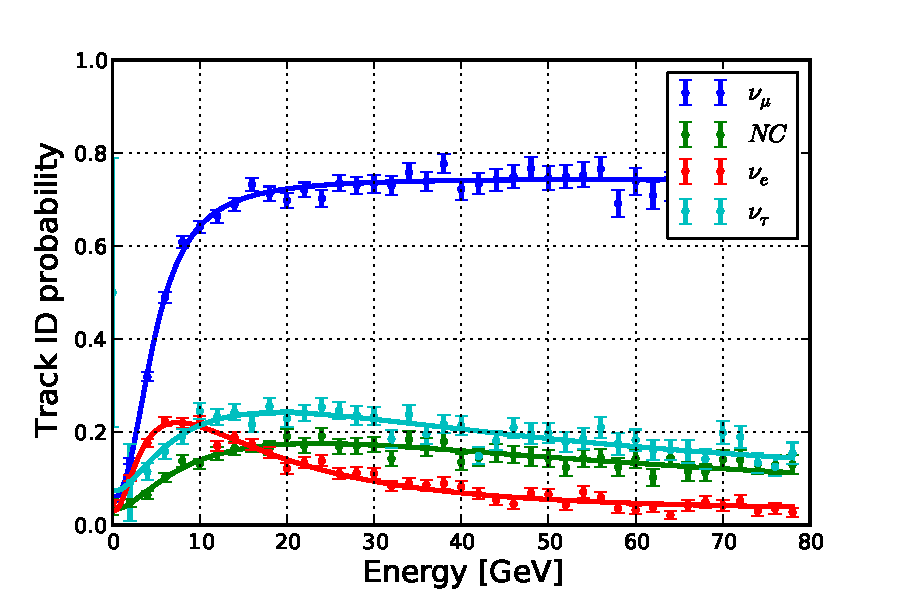
\includegraphics[width=0.7\textwidth]{figures/PID_all.pdf}
%  \caption{Track identification probability as function of energy in all four
%   interaction channels. The straight lines show fits to the data.}
%  \label{fig:PID}
% \end{figure}

